\input{../preamble.tex}

\lecturenumber{12}
\title{Memory}
\version{1.0.0}

\usetikzlibrary{intersections} % /tikz/name path

\tikzset{swapin/.style args = {(#1,#2)}{%
    row #1 column #2/.style={nodes={text=red}}}}

\begin{document}

\begin{frame}[plain, noframenumbering]
    \titlepage
\end{frame}

\begin{slide}

    \slidetitle{Page Allocation Uses A Free List}

    Given physical pages, the operating system maintains a free list (linked
    list)
    \medskip

    The unused pages themselves contain the \texttt{next} pointer in the free list

    \leftspace{}Physical memory gets initialized at boot
    \medskip

    To allocate a page, you remove it from the free list

    \leftspace{}To deallocate a page you add it back to the free list

\end{slide}

\begin{slide}

	\slidetitle{Back to Creating A Process}
	
	A large virtual address space is allocated "for free" to a process.
	
	\vspace{5mm}
	
	Page table?
	
	\vspace{5mm}
	
	RAM allocation?
	
\end{slide}

\begin{slide}

	\slidetitle{Back to Forking A Process}
	
	Copy-on-write
	
	\vspace{5mm}
	
	Page table?
	
	\vspace{5mm}
	
	RAM allocation?
	
\end{slide}

\begin{slide}

    \slidetitle{why do we need to copy the page tables?}

    We don't! There's a system call for that --- \texttt{vfork}
    \bigskip

    \texttt{vfork} shares all memory with the parent 

    \leftspace{}It's undefined behavior to modify anything
    \bigskip

    Only used in very performance sensitive programs

\end{slide}  

\begin{slide}

    \slidetitle{Demand Paging}

    We use memory as a cache for the file system
    \medskip

    Map memory pages to file system blocks

    \leftspace{}Only load them into memory when they're used through
    the page fault handler
    \medskip

    If the page doesn't represent a file, we can map it to swap space

    \leftspace{}Move it to disk if we need to use more physical memory

\end{slide}

\begin{slide}

    \slidetitle{A Processes' Working Set Should Fit in Physical Memory}

    Given an amount of time, the number of pages your process uses
    is called
    its \textit{working set}
    \medskip

    If you cannot fit your working set into physical memory your process
    will \textit{thrash}

    \leftspace{}It's constantly moving entries in and out of cache

\end{slide}

\begin{slide}

    \slidetitle{Not all virtual memory is mapped to physical memory}

    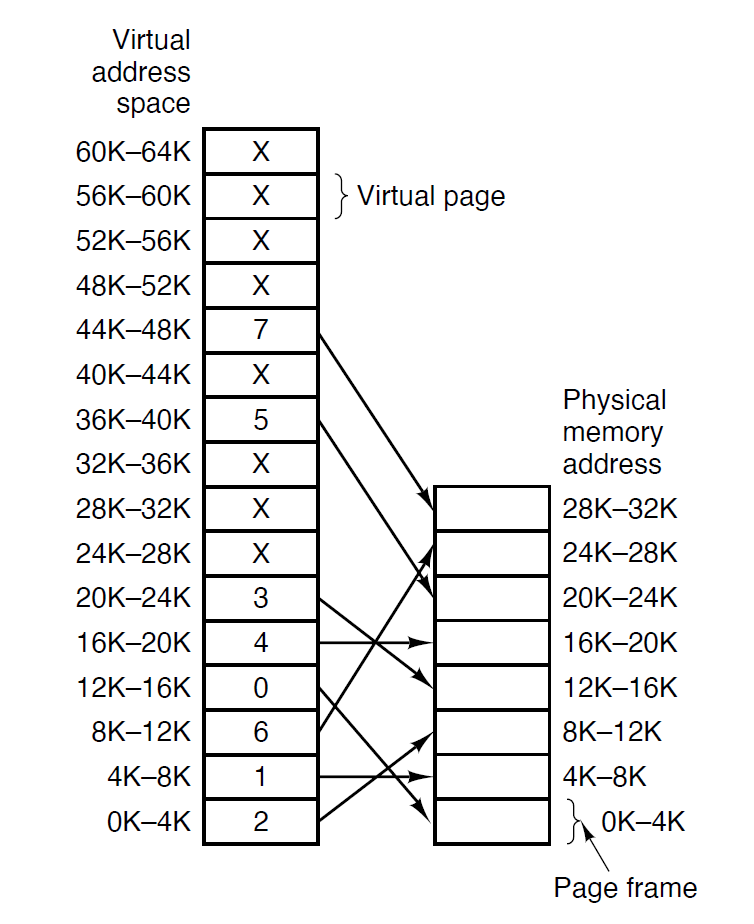
\includegraphics[width=50mm]{unmapped-mem.png}

\end{slide}

\begin{slide}
    
    \slidetitle{What Should We Do About the Page Table Size?}

    Most programs don't use all the virtual memory space, how can we take
    advantage?

\end{slide}
  
\begin{slide}
    
    \slidetitle{We Can Make Our Page Table Fit on a Page}

	\vspace{-8mm}
	
    \centering
    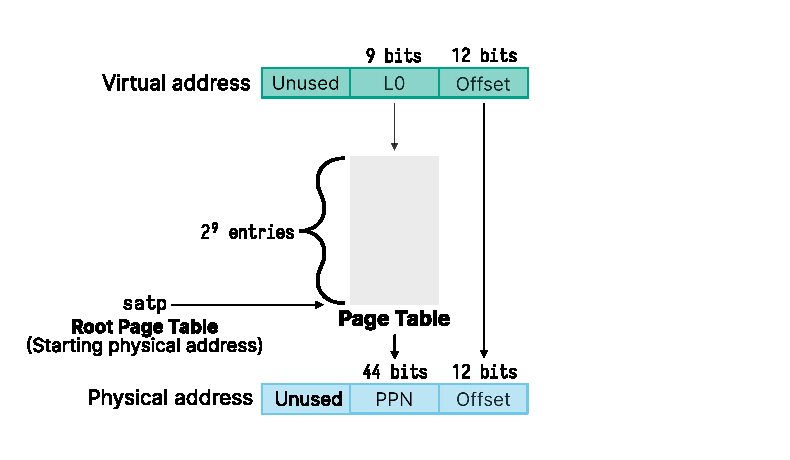
\includegraphics{single-level-page-table-small.eps}

\end{slide}

\begin{slide}

	\vspace{-8mm}
	
    \slidetitle{Multi-Level Page Tables Save Space for Sparse Allocations}

    \centering
    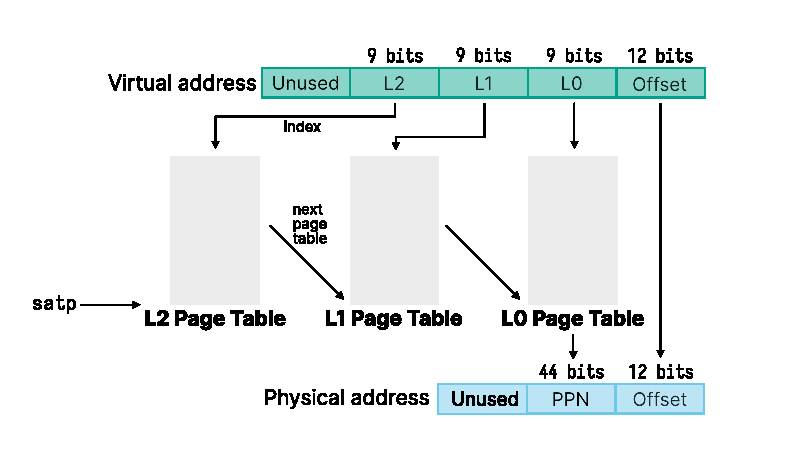
\includegraphics{multi-level-page-table.eps} 

\end{slide}

\begin{slide}

	\slidetitle{Consider Just Two Levels}
	\vspace{-2mm}
	
	Let's consider a 30-bit virtual address with 4kB page. 
	
	\medskip
	
	\begin{minipage}{0.49\textwidth}
		Single-Level Page Table
	\end{minipage}
	\hfill
	\begin{minipage}{0.49\textwidth}
		Multi-Level Page Table
	\end{minipage}
	
\end{slide}

\begin{slide}

    \slidetitle{Consider Just Two Levels}

    Assume our process uses just one virtual address at \texttt{0x3FFFF008}

    \leftspace{}or \texttt{0b11\_1111\_1111\_1111\_1111\_0000\_0000\_1000}

    \leftspace{}or \texttt{0b111111111\_111111111\_000000001000}
    \medskip

    We'll just consider a 30-bit virtual address with a page size of 4096 bytes

    \leftspace{}We would need a 2 MiB page table if we only had one
    ($\mathsf{2^{18} \times 2^{3}}$)
    \medskip

    Instead, we have a 4 KiB L1 page table ($\mathsf{2^9 \times 2^{3}}$) and a 4
    KiB L0 page table

    \leftspace{}Total of 8 KiB instead of 2 MiB
    \medskip

    Note: worst case if we used all virtual addresses we would consume 2 MiB + 4
    KiB

\end{slide}

\begin{slide}

	\slidetitle{Back to \texttt{malloc} and \texttt{free}}
	
	What happens when you \texttt{malloc} memory?
	\vspace{3mm}
	
	If a process “shrinks” its heap at the application level (e.g., via free() calls), does that actually reduce the process’s overall memory usage from the operating system’s perspective?

\end{slide}

\begin{slide}

	\slidetitle{Practice Question}
	
	Consider a system with 4096-byte pages, a PTE size of 6 bytes, 42-bit virtual addresses, and 48-bit physical addresses.
	
	\bigskip
	
	(a) How many offset bits are there in the virtual address?
	
	\medskip
	
	(b) How many bits of the virtual address are left over for index bits?
	
	\medskip
	
	(c) For a single page table, how large would the table need to be? 
		
	\medskip
	
	(d) How many PTEs could fit on a single page?
	
	\medskip
	
	(e) How many levels of page tables would you need to ensure each page table fits on a single page?
	
\end{slide}

\begin{slide}
    
    \slidetitle{Alignment: Memory Eventually Lines Up with Byte 0}

    If pages are \textit{4096 byte aligned} in memory is means pages always
    start when the lower 12 bits are zero, in computing we like alignment
    \medskip

    If a page started at address \texttt{0x7C00} its last byte would be at
    address \texttt{0x8BFF}
    \medskip

    Instead, a page would start at \texttt{0x7000} and end at \texttt{0x7FFF}
    \bigskip

    Question: Is address \texttt{0xEC} 8 byte aligned?
	
\end{slide}

\begin{slide}

	\slidetitle{Alignment Example}
	
	\begin{minted}{c}
struct AlignmentDemo
{
    char char_a;
    int int_a;
    char char_b;
    char char_c;
    char char_d;
    int int_b;
    int int_c;
};
	\end{minted}

\end{slide}

\begin{slide}

    \slidetitle{Using the Page Tables for Every Memory Access is Slow}

    We need to follow pointers across multiple levels of page tables!
    \medskip

    We'll likely access the same page multiple times
    
    (close to the first access time)
    \medskip

    A process may only need a few VPN $\rightarrow$ PPN mappings at a time
    \medskip

    Our solution is another computer science classic: caching

\end{slide}

\begin{slide}

    \slidetitle{A Translation Look-Aside Buffer (TLB) Caches PTEs}
	
	\vspace{-5mm}
	
    \centering
    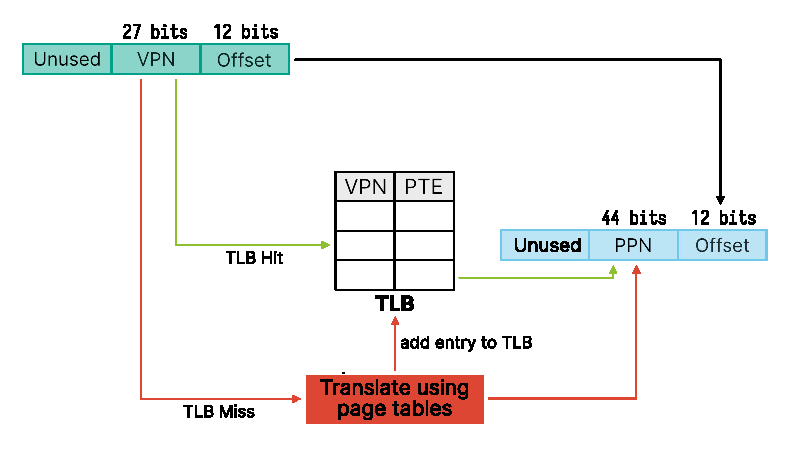
\includegraphics{tlb.eps}

\end{slide}

\begin{slide}

    \slidetitle{Effective Access Time (EAT)}

    Assume a single page table
    
    \leftspace{}(there's only one additional memory access in the page table)
    \medskip

    $\mathsf{TLB\_Hit\_Time = TLB\_Search + Mem}$

    $\mathsf{TLB\_Miss\_Time = TLB\_Search + 2 \times Mem}$

    $\mathsf{EAT = \alpha \times TLB\_Hit\_Time + (1 - \alpha) \times TLB\_Miss\_Time}$
    \medskip

    If $\mathsf{\alpha = 0.8}$, $\mathsf{TLB\_Search = 10\ ns}$, and accesses take 100 ns, calculate EAT

\end{slide}

\begin{slide}

    \slidetitle{Context Switches Require Handling the TLB}

    You can either flush the cache, or attach a process ID to the TLB
    \medskip

    Most implementation just flush the TLB

    \leftspace{}RISC-V uses a \texttt{sfence.vma} instruction to flush the TLB
    \medskip

    On x86 loading the base page table will also flush the TLB

\end{slide}

\begin{slide}
    
    \slidetitle{
      Computer Memory Hierarchy is a
    
      Trade-off of Capacity and Speed
    }

    \centering
	\begin{tikzpicture}[shorten >=0pt, scale=0.9, transform shape]
	  \coordinate (A) at (-5,0) {};
	  \coordinate (B) at ( 5,0) {};
	  \coordinate (C) at (0,7) {};
	  \draw[name path=AC] (A) -- (C);
	  \draw[name path=BC] (B) -- (C);
	  \foreach \y/\A in {
		0/Tape Drives,
		1/Hard Disk Drive (HDD),
		2/SATA Solid State Disk (SSD),
		3/Non-Volatile Memory (NVMe),
		4/Memory (RAM),
		5/CPU Cache,
		6/CPU
	  } {
		\draw ($(A)!\y/7!(C)$) -- ($(B)!\y/7!(C)$)
		  node[midway,above] {\A};
	  }

	  \draw [->, very thick] (-3,6) -- (-3,4) node[midway, left] {Capacity};
	  \draw [->, very thick] (3,4) -- (3,6) node[midway, right] {Speed (and price)};
	\end{tikzpicture}

\end{slide}

\begin{slide}

    \slidetitle{We Want to Hide the Hierarchy from the User}

    Each level wants to pretend it has the speed of the layer above it

    \leftspace{}and the capacity of the layer below it
    \medskip

    The memory used by all the processes my exceed the amount of physical memory

    \leftspace{}Not all of them may be in use at the same time
    \medskip

    Only keep referenced pages in memory, put others on disk

    \leftspace{}Swap pages back to memory when they're needed

\end{slide}

\begin{slide}

    \slidetitle{Page Replacement Algorithms}

    Optimal

    \leftspace{}Replace the page that won't be used for the longest
    \medskip

    Random

    \leftspace{}Replace a random page
    \medskip

    First-in First-out (FIFO)

    \leftspace{}Replace the oldest page first
    \medskip

    Least Recently Used (LRU)

    \leftspace{}Replace the page that hasn't been used in the longest time

\end{slide}

\begin{slide}

    \slidetitle{Page Replacement Evaluation}

    Assume our physical memory can only hold 4 pages, and we access the following:

    \leftspace{}1 2 3 4 1 2 5 1 2 3 4 5 (all of the pages are initially on disk)
    \medskip

    We'll use this for a bunch of examples during this lecture

    \leftspace{}We want the fewest number of page faults
    \medskip

    For every example we'll find the number of page faults

\end{slide}

\begin{slide}

    \slidetitle{Optimal Example}

    Assume our physical memory can only hold 4 pages, and we access the following:

    \leftspace{}1 2 3 4 1 2 5 1 2 3 4 5 (all of the pages are initially on disk)

    \begin{center}
      \begin{tikzpicture}[
        every node/.style={
          align=center,
          text height=2ex,
          text width=1em
        },
        swapin/.list={
          (2,1),
          (3,2),
          (4,3),
          (5,4),
          (5,7),
          (2,11)
        },
      ]
        \matrix (m) [
          matrix of nodes,
          nodes in empty cells,
          column sep=1em,
          column 2/.style={visible on=<2->},
          column 3/.style={visible on=<3->},
          column 4/.style={visible on=<4->},
          column 5/.style={visible on=<5->},
          column 6/.style={visible on=<6->},
          column 7/.style={visible on=<7->},
          column 8/.style={visible on=<8->},
          column 9/.style={visible on=<9->},
          column 10/.style={visible on=<10->},
          column 11/.style={visible on=<11->},
          column 12/.style={visible on=<12->},
        ] {
          1 & 2 & 3 & 4 & 1 & 2 & 5 & 1 & 2 & 3 & 4 & 5 \\
          1 & 1 & 1 & 1 & 1 & 1 & 1 & 1 & 1 & 1 & 4 & 4 \\
            & 2 & 2 & 2 & 2 & 2 & 2 & 2 & 2 & 2 & 2 & 2 \\
            &   & 3 & 3 & 3 & 3 & 3 & 3 & 3 & 3 & 3 & 3 \\
            &   &   & 4 & 4 & 4 & 5 & 5 & 5 & 5 & 5 & 5 \\
        };
        \draw (m-2-1.north west) rectangle (m-5-1.south east);
        \draw (m-2-2.north west) rectangle (m-5-2.south east);
        \draw (m-2-3.north west) rectangle (m-5-3.south east);
        \draw (m-2-4.north west) rectangle (m-5-4.south east);
        \draw (m-2-5.north west) rectangle (m-5-5.south east);
        \draw (m-2-6.north west) rectangle (m-5-6.south east);
        \draw (m-2-7.north west) rectangle (m-5-7.south east);
        \draw (m-2-8.north west) rectangle (m-5-8.south east);
        \draw (m-2-9.north west) rectangle (m-5-9.south east);
        \draw (m-2-10.north west) rectangle (m-5-10.south east);
        \draw (m-2-11.north west) rectangle (m-5-11.south east);
        \draw (m-2-12.north west) rectangle (m-5-12.south east);
      \end{tikzpicture}
    \end{center}

    \begin{flushright}
      \onslide<13->{6 page faults}
    \end{flushright}

\end{slide}

\begin{slide}

    \slidetitle{FIFO Example}

    Assume our physical memory can only hold 4 pages, and we access the following:

    \leftspace{}1 2 3 4 1 2 5 1 2 3 4 5 (all of the pages are initially on disk)

    \begin{center}
      \begin{tikzpicture}[
        every node/.style={
          align=center,
          text height=2ex,
          text width=1em
        },
        swapin/.list={
          (2,1),
          (3,2),
          (4,3),
          (5,4),
          (2,7),
          (3,8),
          (4,9),
          (5,10),
          (2,11),
          (3,12)
        },
      ]
        \matrix (m) [
          matrix of nodes,
          nodes in empty cells,
          column sep=1em,
          column 2/.style={visible on=<2->},
          column 3/.style={visible on=<3->},
          column 4/.style={visible on=<4->},
          column 5/.style={visible on=<5->},
          column 6/.style={visible on=<6->},
          column 7/.style={visible on=<7->},
          column 8/.style={visible on=<8->},
          column 9/.style={visible on=<9->},
          column 10/.style={visible on=<10->},
          column 11/.style={visible on=<11->},
          column 12/.style={visible on=<12->},
        ] {
          1 & 2 & 3 & 4 & 1 & 2 & 5 & 1 & 2 & 3 & 4 & 5 \\
          1 & 1 & 1 & 1 & 1 & 1 & 5 & 5 & 5 & 5 & 4 & 4 \\
            & 2 & 2 & 2 & 2 & 2 & 2 & 1 & 1 & 1 & 1 & 5 \\
            &   & 3 & 3 & 3 & 3 & 3 & 3 & 2 & 2 & 2 & 2 \\
            &   &   & 4 & 4 & 4 & 4 & 4 & 4 & 3 & 3 & 3 \\
        };
        \draw (m-2-1.north west) rectangle (m-5-1.south east);
        \draw (m-2-2.north west) rectangle (m-5-2.south east);
        \draw (m-2-3.north west) rectangle (m-5-3.south east);
        \draw (m-2-4.north west) rectangle (m-5-4.south east);
        \draw (m-2-5.north west) rectangle (m-5-5.south east);
        \draw (m-2-6.north west) rectangle (m-5-6.south east);
        \draw (m-2-7.north west) rectangle (m-5-7.south east);
        \draw (m-2-8.north west) rectangle (m-5-8.south east);
        \draw (m-2-9.north west) rectangle (m-5-9.south east);
        \draw (m-2-10.north west) rectangle (m-5-10.south east);
        \draw (m-2-11.north west) rectangle (m-5-11.south east);
        \draw (m-2-12.north west) rectangle (m-5-12.south east);
      \end{tikzpicture}
    \end{center}

    \begin{flushright}
      \onslide<13->{10 page faults}
    \end{flushright}

\end{slide}

\begin{slide}

    \slidetitle{FIFO Example (3 Page Frames)}

    Assume our physical memory can only hold \textbf{3} pages, and we access the following:

    \leftspace{}1 2 3 4 1 2 5 1 2 3 4 5 (all of the pages are initially on disk)

    \begin{center}
      \begin{tikzpicture}[
        every node/.style={
          align=center,
          text height=2ex,
          text width=1em
        },
        swapin/.list={
          (2,1),
          (3,2),
          (4,3),
          (2,4),
          (3,5),
          (4,6),
          (2,7),
          (3,10),
          (4,11)
        },
      ]
        \matrix (m) [
          matrix of nodes,
          nodes in empty cells,
          column sep=1em,
          column 2/.style={visible on=<2->},
          column 3/.style={visible on=<3->},
          column 4/.style={visible on=<4->},
          column 5/.style={visible on=<5->},
          column 6/.style={visible on=<6->},
          column 7/.style={visible on=<7->},
          column 8/.style={visible on=<8->},
          column 9/.style={visible on=<9->},
          column 10/.style={visible on=<10->},
          column 11/.style={visible on=<11->},
          column 12/.style={visible on=<12->},
        ] {
          1 & 2 & 3 & 4 & 1 & 2 & 5 & 1 & 2 & 3 & 4 & 5 \\
          1 & 1 & 1 & 4 & 4 & 4 & 5 & 5 & 5 & 5 & 5 & 5 \\
            & 2 & 2 & 2 & 1 & 1 & 1 & 1 & 1 & 3 & 3 & 3 \\
            &   & 3 & 3 & 3 & 2 & 2 & 2 & 2 & 2 & 4 & 4 \\
        };
        \draw (m-2-1.north west) rectangle (m-4-1.south east);
        \draw (m-2-2.north west) rectangle (m-4-2.south east);
        \draw (m-2-3.north west) rectangle (m-4-3.south east);
        \draw (m-2-4.north west) rectangle (m-4-4.south east);
        \draw (m-2-5.north west) rectangle (m-4-5.south east);
        \draw (m-2-6.north west) rectangle (m-4-6.south east);
        \draw (m-2-7.north west) rectangle (m-4-7.south east);
        \draw (m-2-8.north west) rectangle (m-4-8.south east);
        \draw (m-2-9.north west) rectangle (m-4-9.south east);
        \draw (m-2-10.north west) rectangle (m-4-10.south east);
        \draw (m-2-11.north west) rectangle (m-4-11.south east);
        \draw (m-2-12.north west) rectangle (m-4-12.south east);
      \end{tikzpicture}
    \end{center}

    \begin{flushright}
      \onslide<13->{9 page faults}
    \end{flushright}

\end{slide}

\begin{slide}

    \slidetitle{Bélády's Anomaly Says More Page Frames Causes More Faults}

    This is a problem with FIFO algorithms

    \leftspace{}Does not exist with LRU or ``stack-based algorithms''
    \medskip

    Paper in 2010 found that this FIFO anomaly is unbounded (\url{https://arxiv.org/abs/1003.1336})

    \leftspace{}You could construct a sequence to get any arbitrary page fault ratio
    \medskip

    For other algorithms:

    \leftspace{}increasing the number of page frames decreases the number of
    page faults

\end{slide}

\begin{slide}

    \slidetitle{LRU Example (Use FIFO to Break Ties)}

    Assume our physical memory can only hold 4 pages, and we access the following:

    \leftspace{}1 2 3 4 1 2 5 1 2 3 4 5 (all of the pages are initially on disk)

    \begin{center}
      \begin{tikzpicture}[
        every node/.style={
          align=center,
          text height=2ex,
          text width=1em
        },
        swapin/.list={
          (2,1),
          (3,2),
          (4,3),
          (5,4),
          (4,7),
          (5,10),
          (4,11),
          (2,12)
        },
      ]
        \matrix (m) [
          matrix of nodes,
          nodes in empty cells,
          column sep=1em,
          column 2/.style={visible on=<2->},
          column 3/.style={visible on=<3->},
          column 4/.style={visible on=<4->},
          column 5/.style={visible on=<5->},
          column 6/.style={visible on=<6->},
          column 7/.style={visible on=<7->},
          column 8/.style={visible on=<8->},
          column 9/.style={visible on=<9->},
          column 10/.style={visible on=<10->},
          column 11/.style={visible on=<11->},
          column 12/.style={visible on=<12->},
        ] {
          1 & 2 & 3 & 4 & 1 & 2 & 5 & 1 & 2 & 3 & 4 & 5 \\
          1 & 1 & 1 & 1 & 1 & 1 & 1 & 1 & 1 & 1 & 1 & 5 \\
            & 2 & 2 & 2 & 2 & 2 & 2 & 2 & 2 & 2 & 2 & 2 \\
            &   & 3 & 3 & 3 & 3 & 5 & 5 & 5 & 5 & 4 & 4 \\
            &   &   & 4 & 4 & 4 & 4 & 4 & 4 & 3 & 3 & 3 \\
        };
        \draw (m-2-1.north west) rectangle (m-5-1.south east);
        \draw (m-2-2.north west) rectangle (m-5-2.south east);
        \draw (m-2-3.north west) rectangle (m-5-3.south east);
        \draw (m-2-4.north west) rectangle (m-5-4.south east);
        \draw (m-2-5.north west) rectangle (m-5-5.south east);
        \draw (m-2-6.north west) rectangle (m-5-6.south east);
        \draw (m-2-7.north west) rectangle (m-5-7.south east);
        \draw (m-2-8.north west) rectangle (m-5-8.south east);
        \draw (m-2-9.north west) rectangle (m-5-9.south east);
        \draw (m-2-10.north west) rectangle (m-5-10.south east);
        \draw (m-2-11.north west) rectangle (m-5-11.south east);
        \draw (m-2-12.north west) rectangle (m-5-12.south east);
      \end{tikzpicture}
    \end{center}

    \begin{flushright}
      \onslide<13->{8 page faults}
    \end{flushright}

\end{slide}

\begin{slide}

    \slidetitle{Implementing LRU in Hardware Has to Search All Pages}

    You could implement it by keeping a counter for each page
    \medskip

    For each page reference, save the system clock into the counter
    \medskip


    For replacement, scan through the pages and find the one with the oldest clock

\end{slide}

\begin{slide}

    \slidetitle{Implementing LRU in Software is Too Expensive}

    Create a doubly linked list of pages
    \medskip

    For each page reference, move it to the front of the list
    \medskip

    For replacement, remove from the back of the list
    \medskip

    It requires 6 pointer updates for each page reference, and

    \leftspace{}also creates a high contention bottleneck for multiple processors

\end{slide}

\begin{slide}

    \slidetitle{Implementing LRU in Practice Isn't Going to Work}

    We settle for approximate LRU

    \leftspace{}LRU is an approximation of the optimal case anyways
    \medskip

    There's lots of different tweaks you can do to implement it more efficiently
    \medskip

    We'll be looking at the clock algorithm, but there's also:

    \leftspace{}Least Frequently Used (LFU), 2Q, Adaptive Replacement Cache (ARC)

\end{slide}

\begin{slide}

    \slidetitle{Implementing LRU in Practice Isn't Going to Work}

    We settle for approximate LRU

    \leftspace{}LRU is an approximation of the optimal case anyways
    \medskip

    There's lots of different tweaks you can do to implement it more efficiently
    \medskip

    We'll be looking at the clock algorithm, but there's also:

    \leftspace{}Least Frequently Used (LFU), 2Q, Adaptive Replacement Cache (ARC)

\end{slide}

\begin{slide}

    \slidetitle{Clock Algorithm}

    Data structures:
    \begin{itemize}
      \item Keeps a circular list of pages in memory
      \item Uses a reference bit for each page in memory (light grey in next slides)
      \item Has a ``hand'' (iterator) pointing to the last element examined
    \end{itemize}
    \medskip

    Algorithm, to insert a new page:
    \begin{itemize}
      \item Check the hand's reference bit, if it's 0 then place the page and advance hand
      \item If the reference bit is 1, set it to 0, advance the hand, and repeat
    \end{itemize}
    \medskip

    For page accesses, set the reference bit to 1

\end{slide}

\begin{slide}

    \slidetitle{Clock Example (with Diagram)}

	\vspace{-5mm}
	
    Assume our physical memory can only hold 4 pages, and we access the following:

    \leftspace{}1 2 3 4 5 2 3 1 2 3 (all of the pages are initially on disk)

	\vspace{-2mm}
	
    \begin{center}
      \begin{tikzpicture}
        \matrix (m) [
          matrix of nodes,
          nodes in empty cells,
          minimum width=2em,
          minimum height=2em,
          align=center,
          column sep=1em,
          column 1/.style={visible on=<2->},
          column 2/.style={visible on=<3->},
          column 3/.style={visible on=<4->},
          column 4/.style={visible on=<5->},
          column 5/.style={visible on=<6->},
          column 6/.style={visible on=<11->},
          column 7/.style={visible on=<12->},
          column 8/.style={visible on=<13->},
          column 9/.style={visible on=<16->},
          column 10/.style={visible on=<17->},
        ] {
          1 & 2 & 3 & 4 & 5 & 2 & 3 & 1 & 2 & 3 \\
        };
      \end{tikzpicture}

      \begin{tikzpicture}[
        box/.style={
          draw,
          align=center,
          minimum width=2em,
          minimum height=6em,
          rectangle split,
          rectangle split parts=2,
          rectangle split part fill={white, black!20},
        }
      ]

        \node (c) at (0, 0) {};

        \node<1> [above=of c, box] (n) {0 \nodepart{second} 0};
        \node<2-5> [above=of c, box] {1 \nodepart{second} 1};
        \node<6-9> [above=of c, box] {1 \nodepart{second} 0};
        \node<10-> [above=of c, box] {5 \nodepart{second} 1};

        \node<1-2> [right=of c, box] (e) {0 \nodepart{second} 0};
        \node<3-6,11-12,16-> [right=of c, box] {2 \nodepart{second} 1};
        \node<7-10,13-15> [right=of c, box] {2 \nodepart{second} 0};

        \node<1-3> [below=of c, box] (s) {0 \nodepart{second} 0};
        \node<4-7,12-13,17-> [below=of c, box] {3 \nodepart{second} 1};
        \node<8-11,14-16> [below=of c, box] {3 \nodepart{second} 0};

        \node<1-4> [left=of c, box] (w) {0 \nodepart{second} 0};
        \node<5-8> [left=of c, box] (w) {4 \nodepart{second} 1};
        \node<9-14> [left=of c, box] (w) {4 \nodepart{second} 0};
        \node<15-> [left=of c, box] (w) {1 \nodepart{second} 1};

        \path [->] (n) edge [bend left] (e)
                   (e) edge [bend left] (s)
                   (s) edge [bend left] (w)
                   (w) edge [bend left] (n);

        \path<1,5,9,15-> [->] (c) edge (n);
        \path<2,6,10-12> [->] (c) edge (e);
        \path<3,7,13> [->] (c) edge (s);
        \path<4,8,14> [->] (c) edge (w);

      \end{tikzpicture}
    \end{center}

\end{slide}

\begin{slide}

    \slidetitle{Clock Example}

    Assume our physical memory can only hold 4 pages, and we access the following:

    \leftspace{}1 2 3 4 5 2 3 1 2 3 (all of the pages are initially on disk)

    \begin{center}
      \begin{tikzpicture}[
        every node/.style={
          align=center,
          text height=2ex,
          text width=1em
        }
      ]
        \matrix (m) [
          matrix of nodes,
          nodes in empty cells,
          column sep=1em
        ] {
          1 & 2 & 3 & 4 & 5 & 2 & 3 & 1 & 2 & 3 \\
          1 & 1 & 1 & 1 & 5 & 5 & 5 & 5 & 5 & 5 \\
            & 2 & 2 & 2 & 2 & 2 & 2 & 2 & 2 & 2 \\
            &   & 3 & 3 & 3 & 3 & 3 & 3 & 3 & 3 \\
            &   &   & 4 & 4 & 4 & 4 & 1 & 1 & 1 \\
        };
        \foreach \x in {1,...,10} {
          \draw (m-2-\x.north west) rectangle (m-5-\x.south east);
        }
      \end{tikzpicture}
    \end{center}

    \begin{flushright}
      6 page faults
    \end{flushright}

\end{slide}

\end{document}

